\documentclass[english,floatsintext,man]{apa6}

\usepackage{amssymb,amsmath}
\usepackage{ifxetex,ifluatex}
\usepackage{fixltx2e} % provides \textsubscript
\ifnum 0\ifxetex 1\fi\ifluatex 1\fi=0 % if pdftex
  \usepackage[T1]{fontenc}
  \usepackage[utf8]{inputenc}
\else % if luatex or xelatex
  \ifxetex
    \usepackage{mathspec}
    \usepackage{xltxtra,xunicode}
  \else
    \usepackage{fontspec}
  \fi
  \defaultfontfeatures{Mapping=tex-text,Scale=MatchLowercase}
  \newcommand{\euro}{€}
\fi
% use upquote if available, for straight quotes in verbatim environments
\IfFileExists{upquote.sty}{\usepackage{upquote}}{}
% use microtype if available
\IfFileExists{microtype.sty}{\usepackage{microtype}}{}

% Table formatting
\usepackage{longtable, booktabs}
\usepackage{lscape}
% \usepackage[counterclockwise]{rotating}   % Landscape page setup for large tables
\usepackage{multirow}		% Table styling
\usepackage{tabularx}		% Control Column width
\usepackage[flushleft]{threeparttable}	% Allows for three part tables with a specified notes section
\usepackage{threeparttablex}            % Lets threeparttable work with longtable

% Create new environments so endfloat can handle them
% \newenvironment{ltable}
%   {\begin{landscape}\begin{center}\begin{threeparttable}}
%   {\end{threeparttable}\end{center}\end{landscape}}

\newenvironment{lltable}
  {\begin{landscape}\begin{center}\begin{ThreePartTable}}
  {\end{ThreePartTable}\end{center}\end{landscape}}




% The following enables adjusting longtable caption width to table width
% Solution found at http://golatex.de/longtable-mit-caption-so-breit-wie-die-tabelle-t15767.html
\makeatletter
\newcommand\LastLTentrywidth{1em}
\newlength\longtablewidth
\setlength{\longtablewidth}{1in}
\newcommand\getlongtablewidth{%
 \begingroup
  \ifcsname LT@\roman{LT@tables}\endcsname
  \global\longtablewidth=0pt
  \renewcommand\LT@entry[2]{\global\advance\longtablewidth by ##2\relax\gdef\LastLTentrywidth{##2}}%
  \@nameuse{LT@\roman{LT@tables}}%
  \fi
\endgroup}


  \usepackage{graphicx}
  \makeatletter
  \def\maxwidth{\ifdim\Gin@nat@width>\linewidth\linewidth\else\Gin@nat@width\fi}
  \def\maxheight{\ifdim\Gin@nat@height>\textheight\textheight\else\Gin@nat@height\fi}
  \makeatother
  % Scale images if necessary, so that they will not overflow the page
  % margins by default, and it is still possible to overwrite the defaults
  % using explicit options in \includegraphics[width, height, ...]{}
  \setkeys{Gin}{width=\maxwidth,height=\maxheight,keepaspectratio}
\ifxetex
  \usepackage[setpagesize=false, % page size defined by xetex
              unicode=false, % unicode breaks when used with xetex
              xetex]{hyperref}
\else
  \usepackage[unicode=true]{hyperref}
\fi
\hypersetup{breaklinks=true,
            pdfauthor={},
            pdftitle={Of waves and peas: Accepting the null across scientific history},
            colorlinks=true,
            citecolor=blue,
            urlcolor=blue,
            linkcolor=black,
            pdfborder={0 0 0}}
\urlstyle{same}  % don't use monospace font for urls

\setlength{\parindent}{0pt}
%\setlength{\parskip}{0pt plus 0pt minus 0pt}

\setlength{\emergencystretch}{3em}  % prevent overfull lines

\ifxetex
  \usepackage{polyglossia}
  \setmainlanguage{}
\else
  \usepackage[english]{babel}
\fi

% Manuscript styling
\captionsetup{font=singlespacing,justification=justified}
\usepackage{csquotes}
\usepackage{upgreek}

 % Line numbering
  \usepackage{lineno}
  \linenumbers


\usepackage{tikz} % Variable definition to generate author note

% fix for \tightlist problem in pandoc 1.14
\providecommand{\tightlist}{%
  \setlength{\itemsep}{0pt}\setlength{\parskip}{0pt}}

% Essential manuscript parts
  \title{Of waves and peas: Accepting the null across scientific history}

  \shorttitle{Historical nulls}


  \author{Richard D. Morey\textsuperscript{1}~\& Saskia Homer\textsuperscript{1}}

  \def\affdep{{"", ""}}%
  \def\affcity{{"", ""}}%

  \affiliation{
    \vspace{0.5cm}
          \textsuperscript{1} School of Psychology, Cardiff University  }

  \authornote{
    \newcounter{author}
    This draft was compiled at Tue Nov 28 10:31:32 2017 (Europe/London).
    Text, code, and data from Michelson and Morley (1887) and Mendel (1866)
    are also available are available at
    \url{https://github.com/richarddmorey/nullHistoryAMPPS}. All figures are
    licensed \href{https://creativecommons.org/licenses/by/4.0/}{CC BY 4.0}.

                      Correspondence concerning this article should be addressed to Richard D. Morey, School of Psychology, 70 Park Place, Cardiff, UK. E-mail: \href{mailto:richarddmorey@gmail.com}{\nolinkurl{richarddmorey@gmail.com}}
                          }


  \abstract{Scientific theories explain phenomena using simplifying assumptions: for
instance, that the speed of light does not depend on the direction in
which the light is moving, or that the height of a pea plant depends on
a small number of alleles randomly obtained from its parents. The
ability to supporting these simplifying assumptions with statistical
evidence is crucial to scientific progress, though it might involve
``accepting'' the null hypothesis. We review two historical examples
where statistical evidence was used to accept a simplifying assumption
(rejecting the luminiferous aether and genetic theory) and one where the
null hypothesis was not accepted in spite of repeated failures
(gravitational waves), drawing lessons from each.}
  \keywords{paper \\

    \indent Word count: 5987
  }





\usepackage{amsthm}
\newtheorem{theorem}{Theorem}
\newtheorem{lemma}{Lemma}
\theoremstyle{definition}
\newtheorem{definition}{Definition}
\newtheorem{corollary}{Corollary}
\newtheorem{proposition}{Proposition}
\theoremstyle{definition}
\newtheorem{example}{Example}
\theoremstyle{definition}
\newtheorem{exercise}{Exercise}
\theoremstyle{remark}
\newtheorem*{remark}{Remark}
\newtheorem*{solution}{Solution}
\begin{document}

\maketitle

\setcounter{secnumdepth}{0}



On a warm summer morning in 1887, Albert Michelson hunched over a heavy
stone table in a basement of Western Reserve College. He peered through
an eyepiece whose other end disappeared under a wooden hood covering the
table. With his right hand, he slowly turned a screw to calibrate one of
sixteen mirrors fixed to the stone. Beneath the hood, beams of yellow
sodium light bounced back and forth between the mirrors along two
perpendicular paths that both ended at the eyepiece. By adjusting the
screw, Michelson ensured that the lengths of the two paths were equal.

The stone slab sat on a piece of wood which itself was floating in a
pool of liquid mercury. Around noon Michelson gave the table a push,
causing it to slowly spin. Every 22.5 degrees of rotation --- about as
many seconds --- he looked through the eyepiece and scribbled down a
number. That afternoon he wrote down over one-hundred readings, stopping
only to give the table a small push to keep it spinning. He came back
that evening for another hundred measurements, repeating the process
again over the next two days.

The numbers Michelson and his colleague Edward Morley scribbled down in
1887 would eventually be among the most celebrated results in science.
What they found --- nothing --- was a quandary for popular nineteenth
century theories of light propagation. Michelson and Morley's (1887)
result foreshadowed not one but \emph{two} revolutions in physics --
special relativity and quantum theory -- and eventually won Michelson
the Nobel prize in physics.

Inferring nothing --- \enquote{accepting the null} as it is sometimes
called --- happens in many contexts in science. One might infer that a
manipulation has no effect. One might also infer support for a theory
from failures to find results that differ very much from a theoretically
predicted value. We present three historical vignettes involving null
inferences (or lack thereof). The first is Michelson and Morley's failed
experiment; the second, Mendel's famous (and controversial) genetic
experiments (Mendel, 1866, Fisher (1936)); and the third, the recent
Nobel-prize-winning findings by the Laser Interferometer
Gravitational-Wave Observatory (LIGO) team. Taken together, these
vignettes offer lessons about null hypotheses in healthy science.

\subsection{Michelson, Morley, and the luminiferous
aether}\label{michelson-morley-and-the-luminiferous-aether}

For many centuries, there were two competing theories explaining the
behavior of light. Emission theory, championed by Newton, held that
light was made up of particles that moved in straight lines called rays.
The opposing view, developed by Huygens, held that light was a wave. In
the eighteenth century, the emission view was dominant. Emission theory
is perhaps most consistent with our everyday observations of light;
light appears to move in straight lines, as a particle would.

In the beginning of the nineteenth century the wave theory of light
gained the upper hand among physicists due to the discovery of
interference phenomena. When two waves of different phases meet, they
cancel and reinforce one another in complicated patterns. Light behaves
this way: when light is forced through slits, the light from one slit
interferes with light from the other, and vice versa. Interference
phenomena cannot be easily explained by an emission theory.

Expectations for light waves were built on other waves that people
understood: waves in water or air. If light was a wave, it must be a
wave in some medium. Whatever this medium is, it carries starlight above
the earth and torchlight below it. It must be able to pass through solid
matter as light moves through glass, and it must exist in a vaccum.
Wave-theorists gave this mysterious medium a name: the
\emph{luminiferous aether}.

Physicists thought that a sea of luminiferous aether existed thoughout
space, providing a fixed reference against which everything moves. As
the earth revolves around the Sun, it is passing through the aether.
Facts known at the time ruled out the idea that the aether was dragged
along with the Earth; hence, the Earth must be moving through the aether
at some speed.

But at what speed? This was the question Michelson and Morley sought to
answer. Michelson had invented and refined an ingeneous experimental
device now known as a Michelson interferometer. The 1887 version is
shown in Figure \ref{fig:MMapp}, in both perspective view (A) and
top-down view (B).

The basic idea behind the Michelson interferometer is that it light
comes from a common source (Figure \ref{fig:MMapp}B, at \(a\)) and is
focused by a lens. The light is split (\(b\)) and sent along two
perpendicular paths, where each beam bounces back and forth between sets
of mirrors. A final mirror along each path (\(e\) and \(e_i\)) sends
each beam back the way it came. The beams are recombined at \(b\) and
pass to the eyepiece (\(f\)). The lengths of the perpendicular paths can
be made equal by carefully adjusting a mirror along one of the paths
(\(e_i\)).

\begin{figure}
\centering
\includegraphics{paper_pdf_files/figure-latex/MMapp-1.pdf}
\caption{\label{fig:MMapp}Michelson and Morley's device (1887, fig. 3 and 4
from the manuscript). A: Perspective drawing of the device without its
wooden cover. The surface was about 1.5m square. B: Schematic of the
table surface. Light emitted from the light source \(a\) through a lens
hits a beam splitter \(b\) and is sent along one of two perpendicular
paths. The light is then reflected back and forth by mirrors at \(d\)
and \(d_i\) (and opposite), until they are reflected back by mirror
\(e\) or \(e_i\). They pass back though the beam splitter and part of
both beams is sent to an eyepiece at \(f\). The mirror \(e_i\) is finely
adjustable so that the two beams can be equated in length. An extra beam
splitter \(c\) is used to ensure that both beams move through the same
amount of glass.}
\end{figure}

When Michelson looked into the eyepiece while he was sending white light
into the interferometer, he saw a pattern of vertical dark and light
bands, called \enquote{fringes}, formed by the interference between the
various components of white light. After calibration, Michelson would
rotate the stone table on which the interferometer was set. If one
imagines the Earth --- and with it, the interferometer --- moving
through the aether, this rotation changes how the two arms are moving
with the aether \enquote{wind}. At some point in the rotation, one arm
will be facing into the wind, and the other arm perpendicular to it; at
another point, the opposite.

The light moves with the aether, but the interferometer itself moves
with the Earth. If one arm is moving parallel to the aether wind and the
other perpendicular to it, the light beams in the two arms move
different distances. Any difference between the arms will cause the
interference fringes to shift to one side by an amount that depends on
the speed of the Earth's motion through the aether. Based on the 30 km/s
speed of the Earth in its orbit, Michelson and Morley expected the
fringes to shift by a maximum of 0.4 fringe widths. This maximum shift
would occur when one arm is facing into the aether wind and the other
perpendicular to it. The minimum shift was 0, when both arms face into
the aether wind at the same angle (see the top of Figure
\ref{fig:MMdata}).

Michelson (or Morley) gave the table a slow but steady spin and measured
the shift at 16 rotation angles, which worked out to once every 23
seconds. They repeated the process consecutively six times, at noon and
in the evening, on three different days. The fringe shift measurements
were detrended to remove the effects of ambient temperature changes, and
then averaged. Michelson and Morley expected a sine curve with amplitude
0.4 fringe widths; Figure \ref{fig:MMdata} shows what they found.

\begin{figure}
\centering
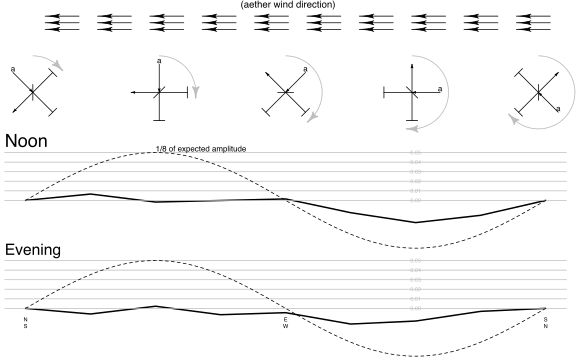
\includegraphics{paper_pdf_files/figure-latex/MMdata-1.pdf}
\caption{\label{fig:MMdata}The data from Michelson and Morley's experiment,
as presented in the manuscript. The top series shows the average of the
detrended noon runs, and the bottom the detrended evening runs. The
\(y\) axis is the amount of shift in fringes. The dotted curve shows the
expected pattern at 1/8 the expected amplitude of 0.4. In the schematic
above, the point marked \enquote{a} represents the light source on the
sketch of the instrument.}
\end{figure}

There does not appear to be any discernable relationship between the
angle of the table's rotation and the fringe shift. There was so little
effect relative to the expected 0.4 fringe shifts that they did not show
the expected effect in their figure at all; the maximum value in their
figure is \emph{1/8} of the predicted value, because showing the
predicted value in the figure would hide all the variability in the
data. In spite of the smallness of the effect, Michelson and Morley did
not directly \enquote{accept} the null. Instead, they say that

\begin{quote}
\enquote{{[}T{]}he displacement to be expected was 0.4 fringe. The
actual displacement was certainly less than the twentieth part of this,
and probably less than the fortieth part. But since the displacement is
proportional to the square of the velocity, the relative velocity of the
earth and the ether is probably less than one sixth the earth's orbital
velocity, and certainly less than one-fourth\ldots{}It appears, from all
that precedes, reasonably certain that if there be any relative motion
between the earth and the luminiferous ether, it must be small\ldots{}}
(Michelson \& Morley, 1887, p.~341)
\end{quote}

Indeed, this result would continue to be refined for decades using more
precise interferometers, and at different times of the year.\footnote{A
  recent replication by Eisele, Nevsky, and Schiller (2009) used an
  interferometer 100 million times as precise as Michelson and Morley's
  device. The result was still null.} Michelson and Morley's result is
remembered as having established that there was no aether. Why is
Michelson and Morley's result considered convincingly null, even though
Michelson and Morley merely report an upper bound on the possible speed
of the Earth moving through the aether?

\textbf{A highly-sensitive experiment.} Michelson and Morley's 1887
experiment was actually the second such experiment that Michelson
published. Michelson (1881) presented similar results, but using a
device 1/10 as sensitive.\footnote{Michelson's 1881 paper is a model of
  scientific transparency. A sizeable portion of the paper is taken up
  describing various difficulties encountered in using his first
  experimental apparatus. Interestingly, although the first paper is
  based on results from a considerably less precise instrument,
  Michelson's earlier conclusions are more definitive: \enquote{The
  interpretation of these results is that there is no displacement of
  the interference bands. The result of the hypothesis of a stationary
  ether is thus shown to be incorrect, and the necessary conclusion
  follows that the hypothesis is erroneous.}} Other researchers noted
that even before accounting for a calculation mistake, \enquote{{[}the
fringe shift{]} to be measured\ldots{}was already barely beyond the
limits of the errors of experiment} and hence \enquote{the conclusion
drawn\ldots{}might well be questioned.} Hence Michelson and Morley's
1887 experiment was designed as a more sensitive replication. In sample
size terms, the relative sensitivity of the 1887 device is akin to
increasing the sample size by a factor of 100. Thankfully, this was
possible due to a clever arrangement of mirrors, and not a 100-fold
increase in costs. The resulting high sensitivity made for a more
convincing null result.

\textbf{A parametric manipulation.} When we discuss null results in
psychology, we often refer to a single effect that is not statistically
significant. Michelson and Morley, however, were looking for a data
pattern, rather than a single effect. The sine wave pattern expected due
to the rotation of the table --- a parameteric manipulation of the size
of the expected \enquote{effect} --- did not present itself. The test of
the theory was therefore much stronger than it would have been if only
one rotational angle had been considered.

\textbf{A theoretical expectation.} The speed of the earth moving around
the sun provided a value against which the null result could be
compared. Michelson and Morley admit that it is possible that other
motion might come into play besides the Earth moving around the sun ---
for instance, the sun moving through the galaxy --- but to get such a
null result, these motions would all have to add up \emph{just right} to
cancel out. This would be quite the coincidence, and so Michelson and
Morley conclude that \enquote{chances are much against it.} They note,
however, that repeating the experiment at longer time intervals would
allow testing this possibility.

\textbf{Competing theories.} As previously mentioned, in the nineteenth
century the wave theory of light was dominant, but was not the only
theory. The competing emission theory had no need for aether. Emission
theory continued to be modified to account for new evidence into the
late nineteenth and early twentieth century (e.g. Ritz, 1908).

Additionally, neither of the two major twentieth century theories in
physics required the luminiferous aether. Einstein's special theory of
relativity (Einstein, 1905) made the aether redundant, and quantum
electrodynamics (Feynman, 1985) accounted for all the wave properties of
light without needing a propagation medium.

These four factors --- the highly-sensitive experiment, the parametric
manipulation of the expected effect, a result far below a theoretical
expectation, and competing theories able to account for the effect ---
combine to create the most important null result in the history of
science. In making the luminiferous aether unnecessary, Michelson and
Morley's results allowed physics move forward without it.

\subsection{Nuller than null: the case of Mendel and
Fisher}\label{nuller-than-null-the-case-of-mendel-and-fisher}

Gregor Mendel, a monk of seemingly impeccable character, conducted his
famous experiments on peas over the years from 1856 to 1863. The
painstaking task of breeding thousands of plants and carefully
classifying their offspring paid off when the resulting data provided
evidence that genetic traits were passed on in discrete forms. Mendel's
evidence was close agreement of the data from his pea plants with his
theory's predictions (Mendel, 1866).

Although Mendel's work on inheritance filled a key gap in nineteenth
century biological understanding, it went largely unnoticed until the
turn of the twentieth century when his results were rediscovered by
several biologists (Piegorsch, 1990). The rediscovery sent ripples
through the genetics community due to its theoretical importance. A
small number of readers, however, noticed something else. Statistically
speaking, the results were good; \emph{surprisingly} good, in fact.

Should a good fit to a true theory be surprising? As Pilgrim (1984) puts
it, \enquote{Mendel's results agreed with his theory. Why shouldn't
they, since his theory was correct?} Fisher (1936) took a different
view. He believed the results were \emph{too} good, and that this was
evidence of falsification. Even worse, Fisher suggests that this
possibly \enquote{contravene{[}s{]} the weight of the evidence supplied
in detail by his paper as a whole} (p.~132). This is not to say Mendel
was wrong, but that his results --- which we review subsequently ---
were not as evidentiary as they might initially appear.

Mendel's experiments considered seven traits of the garden pea plant.
Pea plants, like all living things, have visible traits called
phenotypes that are defined by genes. For instance, a pea plant's seeds
might be round or wrinkled, depending on its genes. These genes come in
pairs --- one from each parent --- and can be of different forms, called
alleles.

A dominant allele can override a recessive allele such that an organism
with both types of allele will have the dominant trait. The round seed
shape is dominant over the wrinkled shape. This means a seed with one of
each allele, called heterozygous, will be round. The three possible
genotypes and their corresponding phenotypes are shown in Figure
\ref{fig:MendelKey}.

\begin{figure}
\includegraphics[width=2.42in]{../../figures/img/Fig1IconKey} \caption{All possible genotypes and corresponding phenotypes for the seed shape trait. Seed shape has two possible alleles (round and wrinkled) and the round allele is dominant. Icons for the genotypes (black-and-white) and phenotypes (solid black) are shown here and used in subsequent figures. The circle denotes the round allele and the star, the wrinkled allele.}\label{fig:MendelKey}
\end{figure}

Mendel theorised there was a 50\% chance of a parent passing each of its
two alleles to its offspring. This leads to easily predictable genotypic
ratios for the seed shape of offspring from two heterozygous parents
(shown in Figure \ref{fig:MendelGenes}).

\begin{figure}
\includegraphics[width=5.68in]{../../figures/img/Fig2GeneEx} \caption{An example of Mendelian genetics with two heterozygous parents (left and top of each square). Inside the squares are the four crossings of the two alleles from each parent. A: The genotype of each possible cross. B: The phenotype of each possible cross. Although 50\% of the alleles correspond to the wrinkled phenotype, only 25\% of the resulting plants will be wrinkled due to the wrinkled allele's recessiveness.}\label{fig:MendelGenes}
\end{figure}

The key to Mendel's experiments were the ratio of phenotypes from
crossings of different plants. Mendel could infer that a plant was
heterozygous if, as a seed, it was round, yet some of its seeds were
wrinkled. Wrinkled-seed offspring are a giveaway that the parent plant
must be passing on a recessive allele, and hence it \emph{must} be
heterozygous. As Figure \ref{fig:MendelGenes} shows, if one crosses a
heterozygous plant with itself, Mendel's theory predicts that 75\% of
the seeds should be round.

\begin{table}[tbp]
\begin{center}
\begin{threeparttable}
\caption{\label{tab:mendel1}Seed totals, $N$, and counts of seeds with the dominant phenotype, $y$, for the seed shape and seed colour experiments taken from Mendel (1886); $p$ is the theoretical proportion of seeds with the dominant phenotype predicted by Mendel's theory; z is the number of theoretical standard deviations between the expected count and observed count.}
\begin{tabular}{llllllll}
\toprule
 & \multicolumn{1}{c}{$p$} & \multicolumn{1}{c}{$N$} & \multicolumn{1}{c}{$y$} & \multicolumn{1}{c}{$Np$} & \multicolumn{1}{c}{$y - Np$} & \multicolumn{1}{c}{$SD(y - Np)$} & \multicolumn{1}{c}{$z=(y-Np)/SD(y - Np)$}\\
\midrule
Shape & 0.75 & 7,324 & 5,474 & 5,493.00 & -19.00 & 37.06 & -0.51\\
Colour & 0.75 & 8,023 & 6,022 & 6,017.25 & 4.75 & 38.79 & 0.12\\
\bottomrule
\end{tabular}
\end{threeparttable}
\end{center}
\end{table}

Table \ref{tab:mendel1} shows the Mendel's results from crossing
heterozygous plants. Of 7324 seeds, we would expect 5493 to be round.
Mendel reports that 5474 were round, only 19 round seeds from the number
expected. Of course, the results of such experiments are variable: if
Mendel is right, the standard deviation of the number of round seeds of
7324 is \(\sqrt{7324 \times .75 \times .25} \approx 37\). Mendel's
results are only half a standard deviation from the theoretical value.
By itself, this closeness is not enough to raise suspicion: there would
be a fair chance --- 38\% --- of obtaining a closer result under
Mendel's theory.

In 1936, Fisher considered all of Mendel's experiments. For every
experiment, we can compute a deviation from the theoretical value, in
standard errors. Because we are interested in the overall
\emph{distance} from the theoretical value, we square every deviation
and sum them across all experiments. The result can be thought of as a
squared distance, in standard errors, from the theoretical value. For
round/wrinkled experiment considered above, we results were \(z_1=.51\)
standard errors below the theoretical value. In a second experiment,
Mendel found that 6022 of 8023 seeds contained yellow, rather than
green, seed leaves. The expected proportion was 75\%, or about 6017
yellow leaves. This observation is five above what was expected, a mere
\(z_2=.12\) standard errors from the theoretical value.

We might think of the theoretical value like the bull's eye of a target,
as shown in Figure \ref{fig:MendelTarget}A. The natural metric of the
target is given by the expected variability of the estimate of the
proportion, the standard error. The figure shows the standard errors as
circles around the bull's eye. To assess how close our two experiments
are to the bull's eye, we work out the distance from the center to the
point (.51, .12), the number of standard errors our two experiments are
away from the theoretical. In the case of our two experiments, this can
be found by the familiar Pythagorean theorem: \(\sqrt{.28}\).

\begin{figure}
\centering
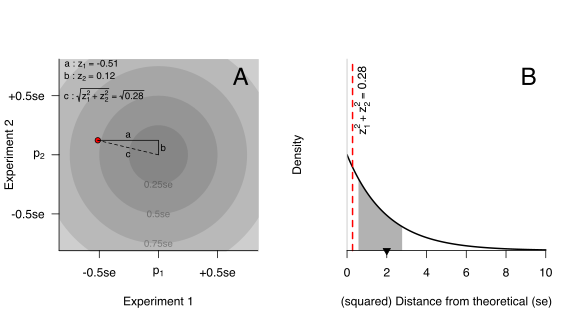
\includegraphics{paper_pdf_files/figure-latex/MendelTarget-1.pdf}
\caption{\label{fig:MendelTarget}A: Calculating the distance, in standard
errors, of a pair of estimates (red circle) from the theoretical values
(center of the bull's eye). Diamonds on the axes show the individual
observations in each experiment. B: The distribution of the squared
distance, assuming two points. The expected squared distance is 2, as
shown by the triangle on the bottom axis. The probabilty of getting a
smaller squared distance than the one observed is about .13, assuming
Mendel's theory. The shaded region shows the middle 50\% of the
distribution.}
\end{figure}

The distance by itself does not tell us whether the results are
surprisingly close; to do this, Fisher compared the observed values to
the sampling distribution under Mendel's theory. If Mendel was right,
the squared distance for two points has a \(\chi^2\) distribution with
two degrees of freedom, as shown in Figure \ref{fig:MendelTarget}B. For
each dimension (here, seed shape and color) we expect to be somewhat off
center. The more dimensions the greater the expected distance, because
each dimension contributes to the distance from the center. The expected
squared distance for two experiments is 2 (these are the degrees of
freedom of the \(\chi^2\)). The \emph{observed} squared distance is much
smaller: .28. Our observed distance from the bull's eye is closer than
what we would expect 87\% of the time, if Mendel's theory is correct.
While far from definitive, this seems close enough to cause some
suspicion. But this analysis only includes two of the 84 experiments
reported by Mendel.

\begin{figure}
\centering
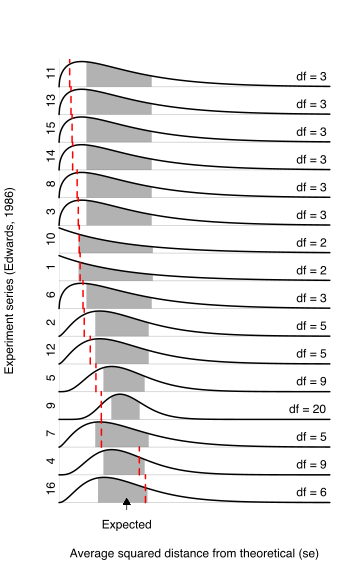
\includegraphics{paper_pdf_files/figure-latex/MendelChi216-1.pdf}
\caption{\label{fig:MendelChi216}Results from Edwards' (1986) sixteen
groupings of Mendel's 84 experiments, along with theoretical
distributions. The series are sorted by deviation from expectation, and
scaled by expectation (degrees of freedom) in order to visually align
all the results. Shaded regions show the middle 50\% of the
distributions.}
\end{figure}

\begin{figure}
\centering
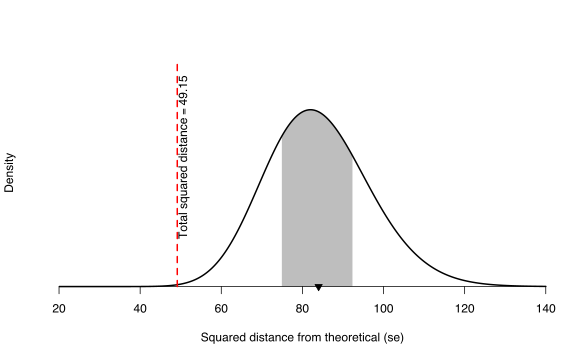
\includegraphics{paper_pdf_files/figure-latex/MendelChi2DF84-1.pdf}
\caption{\label{fig:MendelChi2DF84}Theoretical distribution across all 84
experiments. The red line indicates the observed total squared distance
49.15 (calculated from Edwards' 1986 data). There is a 99.9\% chance
that a random value from this distribution would be larger than 49.15.
The shaded region shows the middle 50\% of the distribution and its
expectation is indicated by the triangle on the bottom axis.}
\end{figure}

Fisher tabulated the results of all 84 Mendel's experiments. For clarity
of presentation, in Figure \ref{fig:MendelChi216} we have grouped the
related results into the 16 series suggested by Edwards (1986) (Table 2,
pp.~306-308), ranging from 2 to 20 degrees of freedom.\footnote{The two
  experiments we considered are series 1 in Figure
  \ref{fig:MendelChi216}. The results are not exactly the same as shown
  in Figure \ref{fig:MendelTarget}B due to the fact that Edwards (1986)
  has removed data that were used in another series in order to make the
  data in each experiment independent from the others. This also causes
  the overall test of all 84 experiments to be different from that
  computed by Fisher, but the difference does not affect the
  conclusions. See Edwards (1986) pp.~299-300.} Notice how most of the
squared distances from the theoretical predictions seem to be on the low
side, closer to 0 than what we would expect. Across all 84 of Mendel's
experiments, we would expect on average a squared distance of 84. The
observed squared distance is substantially less: 49.15. To understand
how small this value is, Figure \ref{fig:MendelChi2DF84} shows a
\(\chi^2\) distribution with 84 degrees of freedom, the sampling
distribution of the squared distance across all experiments assuming
Mendel's theory. The observed distance is so small that we would expect
99.9\% of such sets of experiments to yield a larger distance. The
experiments are \emph{very close} to the theoretical values.

So what? Is Weldon (1902) right when he says that Mendel's results
\enquote{admirably in accord with his experiment} (p.~235)? Is Pilgrim
(1984) right to wonder what the fuss is all about that results closely
agree with a theory? Or is Fisher right when he suggests that
\enquote{most, if not all, of the experiments have been falsified so as
to agree closely with Mendel's expectations} (1936, p.~132)? \emph{Do
results that agree too closely with a theoretical null actually
undermine the evidence}?

The last prominant statistician to weigh in on the debate was Edwards
(1986), who said that

\begin{quote}
\enquote{If it were just a question of having hit the bull's eye with a
single shot we might conclude {[}\ldots{}{]} that Mendel was simply
lucky, but when a whole succession of shots comes close to the bull's
eye we are entitled to invoke skill or some other factor.} (Edwards,
1986, p. 303)
\end{quote}

Of course \enquote{skill} cannot overcome the problem of inherent random
variability. Both Edwards\footnote{Interesting and relevant to the
  modern debate over significance testing is the fact that even the
  likelihoodist Edwards was persuaded by Fisher's logic, in spite of his
  skepticism of significance tests. He said that \enquote{{[}i{]}t may
  be helpful if I admit at this point that for many years I supposed
  that Fisher's analysis was going to be able to be faulted because of
  its total reliance on the \enquote{repeated sampling} logic of the
  \(X^2\) goodness-of-fit test which I had come to mistrust, but a
  complete review of the whole problem has now persuaded me that his
  \enquote{abominable discovery} must stand.} (1986, p.~310)} and more
recently Franklin (2008) suggest that Fisher's analysis has stood the
test of time: Mendel's results are too good to be true. Yet the
controversy is largely unknown outside of statistical circles. Why?

\textbf{Justified suspicion that a result is tainted does not mean it is
wrong.} We are in the lucky position a century and a half later of
knowing that Mendel was right. Science is not always neat; biases will
creep into even the most rigorous research, if only because it is
scientific progress requires interpreting the results of experiments
\emph{post hoc} with incomplete information. As (Dobzhansky, 1967) wrote
at the centennial of Mendel's publication,

\begin{quote}
\enquote{Few experimenters are lucky enough to have no mistakes or
accidents happen in any of their experiments, and it is only common
sense to have such failures discarded. The evident danger is ascribing
to mistakes and expunging from the record perfectly authentic
experimental results which do not fit one's expectations.} (Dobzhansky,
1967, p.~1588)
\end{quote}

Luckily Mendel described his experiments in sufficient detail that they
can be easily repeated. Doubt about any claim can be put to rest by
rigorous replication of the procedure, provided that the theory is
defined clearly enough to decide what a \enquote{replication} would be.

\textbf{Interpretation of results occurs in the context of scientific
theory.} This seems especially obvious in the case of Mendel, given that
the null was derived from Mendel's theory. But suppose Mendel were a
fair-minded experimentalist, and we could travel back in time and
confront him with Fisher's findings? Should Mendel abandon his theory?
Probably not. Although Fisher's critique threatens the evidential force
of Mendel's experiments, Fisher (1936) himself points out that Mendel,
or anyone else in the nineteenth century, could have derived genetic
theory from three simple postulates (1936, pp.~123-124); he also
believed that Mendel may have done so. Fisher thought it possible that
Mendel's experiments were a \enquote{carefully planned demonstration of
his conclusions} (Fisher, 1936, p. 124), rather than their sole support.

\subsection{Unbelievable nulls: LIGO and gravity
waves}\label{unbelievable-nulls-ligo-and-gravity-waves}

Michelson's experiments using interferometers were not only important
for their results; the Michelson interferometer is a tool that continues
to be used in research. Michelson's interferometers were about 1 meter
wide. Modern interferometers range from palm-sized and small enough to
fit in a satelite (Shepherd et al., 1993) to the immense Laser
Interferometer Gravitational-Wave Observatory (LIGO). The LIGO project
operates two interferometers, each with arms 4 km long.\footnote{Even
  LIGO will soon be eclipsed: the European Space Agency plans three
  satelites that will form an gravitational-wave-detecting
  interferometer with arms 2.5 \emph{billion} meters long, called the
  Laser Interferometer Space Antenna (LISA). Imagine Michelson's
  astonishment if he learned that the fiddly instrument with which he
  struggled in a Potsdam cellar would one day be built on an
  interplanetary scale.}

The purpose of LIGO is not to find evidence for the luminiferous aether;
rather, the LIGO team is hunting for gravitational waves. In Einstein's
general theory of relativity, gravity is the result of changes in the
geometry of space-time: a mass, such as a star, bends space-time around
it. When masses accelerate in certain ways --- for example, black holes
orbiting one another --- these distortions are supposed to cause
gravitational waves that propagate away from the source.

The search for gravitational waves serves two purposes: as a test of
general relativity, and as new way of conducting astronomy. We can use
gravity waves in much the same way as we use x-ray, visible-light,
microwave, and radio astronomy to piece together a picture of the
history of the universe. Unlike light, however, gravitational waves are
difficult to detect, because they involve extraordinarily subtle effects
as they pass.

This is where Michelson's interferometer plays a key role. Laser light
is split, shot down the 4 km length of the two arms, bounced back from
precisely suspended mirrors. The laser light is recombined and passed to
a detector. If the arms are the same length, the two recombined waves
cancel; no laser light is detected. When a gravitational wave passes an
interferometer, the two perpendicular arms will change lengths (Figure
\ref{fig:LIGOapp1}). If one arm is longer than the other, then the
cancelation is imperfect and some of the light makes it to the detector.
Space-time distortion from a passing gravitational wave shows up as
fluctuations in the amount of laser light at the detector.

\begin{figure}
\centering
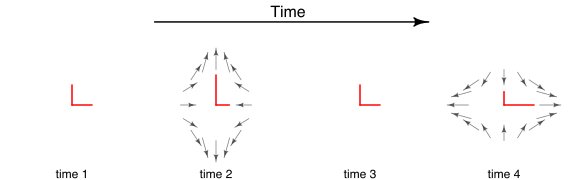
\includegraphics{paper_pdf_files/figure-latex/LIGOapp1-1.pdf}
\caption{\label{fig:LIGOapp1}How gravitational waves distort the length of
the two perpendicular arms of the LIGO Michelson interferometers.}
\end{figure}

Because fluctuations can happen for reasons other than gravitational
waves, LIGO uses multiple sites to crosscheck its results: one in
Washington and one in Louisiana. LIGO also cooperates with the smaller,
3 km Virgo interferometer in Italy (Figure \ref{fig:LIGOapp2}). The LIGO
team looks for \enquote{unusual} events that occur across the detectors.
Looking for correlations across these sites allows noisy fluctuations in
only one detector to be discounted.

\begin{figure}
\centering
\includegraphics{paper_pdf_files/figure-latex/LIGOapp2-1.pdf}
\caption{\label{fig:LIGOapp2}Locations of the Laser Interferometer
Gravitational-Wave Observatory (LIGO) sites in the United States, and
the Virgo interferometer in Italy.}
\end{figure}

LIGO's first attempt at detecting gravitational waves in 2002 yielded a
null result: that is, it was deemed consistent with background noise
(LIGO Scientific Collaboration, 2004). Interestingly, this was expected;
the first run was before the detectors were at full sensitivity. The
introduction to the paper is worth quoting directly:

\begin{quote}
\enquote{The first detection of gravitational wave bursts requires
stable, well understood detectors, well-tested and robust data
processing procedures, and clearly defined criteria for establishing
confidence that no signal is of terrestrial origin. None of these
elements were firmly in place as we began this first LIGO science run;
rather, this run provided the opportunity for us to understand our
detectors better, exercise and hone our data processing procedures, and
build confidence in our ability to establish the detection of
gravitational wave bursts in future science runs. Therefore, the goal
for this analysis is to produce an upper limit on the rate for
gravitational wave bursts, even if a purely statistical procedure
suggests the presence of a signal above background.} (LIGO Scientific
Collaboration, 2004, pp. 102001--3)
\end{quote}

Unlike Michelson's conclusion from his 1881 experiment, the LIGO team
was unwilling to accept the null on the basis of a noisy experiment;
like Michelson and Morley's 1887 experiment, the LIGO state their
results in terms of placing an upper limit on a quantity of
interest.\footnote{It is difficult to imagine a prominent psychology
  journal publishing a null result from an experiment whose purpose is
  to advance understanding of a methodology. Such a result would almost
  certainly be rejected as unimportant.}

From the first failure followed more failures. Six more runs over more
than a decade would yield no evidence --- at least none the team was
willing to accept as inconsistent with background noise --- of
graviational waves. LIGO became \enquote{advanced LIGO} as the team
improved the sensitivity of their instruments. With each failure using a
more sensitive device, a new upper limit was established. The titles
tell the story: \enquote{Upper limits on gravitational-wave bursts in
LIGO's second science run} (The LIGO Scientific Collaboration, 2005);
\enquote{Upper limits on gravitational wave emission from 78 radio
pulsars} (LIGO Scientific Collaboration, 2007); \enquote{Improved Upper
Limits on the Stochastic Gravitational-Wave Background from 2009-2010
LIGO and Virgo Data} (LIGO and Virgo Collaboration, 2014). This work
spawned about 100 papers from 2004 to 2016, characterizing the
instruments, algorithms and their improvements, or presenting data from
their science runs.

Finally, in 2016 the team published a paper announcing the detection of
gravitational waves from the merger of two black holes (LIGO Scientific
Collaboration and Virgo Collaboration, 2016). We are more interested in
what happened in the years before the detection. Why were the LIGO team
unwilling to accept the null and hence the possibility that there were
no gravitational waves? What was the difference between Michelson and
Morley's situation in the late 19th century and the LIGO team's
situation in the early 21st? We believe there are several.

\textbf{The prospect of more sensitive experiments.} The LIGO team was
constantly improving their instruments, and knew that more sensitive
tests were just around the corner.

\textbf{Strong theoretical expectations and low sensitivity} The LIGO
team knew early on that their instruments were not sensitive enough to
detect many gravitational wave events of interest, should they exist.
Unlike Michelson and Morley, LIGO's null results were not unexpected
from the theory.

\textbf{No theoretical rival.} Einstein's general theory of relativity
has withstood numerous tests over the past century. There is no rival to
the theory that could take its place should gravitational waves not
exist. Plunging a field into crisis is not something to be taken
lightly, particularly at the expense of such a well-established theory.

These three conditions made the acceptance of the null hypothesis
difficult, even on the basis of multiple \enquote{failed} LIGO runs.
Luckily, the persistence paid off. Since the 2016 detection, the team
has made several new detections. The ability to consistently detect and
characterize gravitational waves has the potential to usher in a new era
of gravitational wave astronomy, which would not have happened if the
team had accepted the null and given up.

\subsection{Conclusion}\label{conclusion}

We have explored three famous experiments. Michelson and Morley's null
result is understood as having truly shown that a theoretical
light-propagation medium, the luminiferous aether, was unsupported and
unnecessary. Mendel presented a failure to find deviations from
theoretical values, but Fisher noted that these results were actually
\emph{too close} to their theoretical values, calling the evidential
value of the data into doubt. Finally, the LIGO team failed many times
over more than a decade to detect gravitational waves, but never claimed
evidence that gravitational waves do not exist. Eventually detecting
gravitational waves won them the Nobel prize in physics in 2017. We can
take several lessons from these three cases.

\textbf{\enquote{Accepting the null} is not a purely statistical affair;
it occurs in a theoretical context.} Michelson and Morley's result
appeared more compelling because an alternative to wave theory could
account for the result. On the other hand, there is no alternative to
general relativity, so the lack of gravitational waves would throw
physics into crisis. Mendel could have derived his predictions from
three simpler theoretical postulates, and rather tham from the data
themselves. In all three cases, the evidential value of the data was
considered along with higher-level theoretical concerns.

\textbf{Distinguishing between null and small effects requires repeated,
careful, high-sensitivity experiments.} All three groups of
experimenters --- Michelson and Morley, Mendel, and the LIGO team ---
are celebrated for their careful experimentation. Michelson invented
multiple iterations of his device to reduce the noise in his
measurements. Mendel grew thousands of pea plants across 84 experiments
to demonstrate his theory. The LIGO team invested a decade honing their
experimental skills before finding a single gravitational wave. Recently
some have worried that demanding high precision experiments will slow
down scientific progress. We worry that scientific progress isn't
possible without high-precision experiments. Admittedly,
high-sensitivity experiments can be difficult in psychology due to both
resource constraints and natural, poorly-understood human variability.
Advances in research methods, practices, and attitudes --- both
statistical and more broadly --- are needed to overcome these
limitations.

\textbf{Demonstration of positive effects requires the same rigor.} When
interpreting both negative results and positive results, rigor is
critical. The role of potential experimental error in interpreting
negative results was highlighted by Mitchell (2014), who claimed that
this possibility threatened the interpretation of negative replications
(and by extension, negative results in general):

\begin{quote}
\enquote{Because experiments can be undermined by a vast number of
practical mistakes, the likeliest explanation for any failed replication
will always be that the replicator bungled something along the way.
Unless direct replications are conducted by flawless experimenters,
nothing interesting can be learned from them.} (p.~1)
\end{quote}

Indeed, Michelson's initial 1881 null result needed to be replicated
with a more reliable apparatus. If a high-precision replication were not
performed, Michelson's result would have been ignored.

But this raises a critical question: if we do not trust that our
colleagues were thorough and careful when they present us with negative
results, why then do we trust them when they present us with positive
results? Obtaining a positive result does not mean we are off the hook:
detection of gravitational waves was claimed by the BICEP2 team in 2014
(BICEP2 Collaboration et al., 2014). However, the result are now
generally regarded as being confounded by galactic dust (Cowen, 2015).
The BICEP2 team was right --- gravitational waves do exist --- but their
experiment did not demonstrate it. The Nobel prize in physics went to
the LIGO team.

Collectively, the historic results of Michelson and Morley, Mendel, and
the LIGO team show the importance of careful acceptances of null
hypotheses in science. Michelson and Morley's null result allowed
physics to move beyond the concept of a light-propagation medium.
Mendel's null deviations from his theoretical predictions, flawed as
they are, remain among the most celebrated findings in biology. The LIGO
team's null results were part of a larger programme to develop the
experimental tools they needed for the finding that eventially won them
the highest prize in science. Carefully-interpreted null results are not
failures, and should not be doomed to the file-drawer; in any healthy
research programme, they must play a central role.

\newpage

\section{References}\label{references}

\setlength{\parindent}{-0.5in} \setlength{\leftskip}{0.5in}

\hypertarget{refs}{}
\hypertarget{ref-BICEP2:2014}{}
BICEP2 Collaboration, Ade, P., Aikin, R., Barkats, D., Benton, S.,
Bischoff, C., \ldots{} Duband, L. (2014). Detection of \({B}\)-Mode
Polarization at Degree Angular Scales by BICEP2. \emph{Physical Review
Letters}, \emph{112}(24), 241101. Retrieved from
\url{https://link.aps.org/doi/10.1103/PhysRevLett.112.241101}

\hypertarget{ref-Cowen:2015}{}
Cowen, R. (2015). Gravitational waves discovery now officially dead.
\emph{Nature News}. Retrieved from
\url{http://www.nature.com/news/gravitational-waves-discovery-now-officially-dead-1.16830}

\hypertarget{ref-Dobzhansky:1967}{}
Dobzhansky, T. (1967). Looking back at Mendel's discovery.
\emph{Science}, \emph{156}, 1588--1589.

\hypertarget{ref-Edwards:1986}{}
Edwards, A. W. F. (1986). Are Mendel's results really too close?
\emph{Biological Reviews}, \emph{61}, 295--312.

\hypertarget{ref-Einstein:1905}{}
Einstein, A. (1905). Zur elektrodynamik bewegter körper {[}On the
Electrodynamics of Moving Bodies; M. Saha, trans.{]}. \emph{Annalen Der
Physik}, \emph{17}, 891--921.

\hypertarget{ref-Eisele:etal:2009}{}
Eisele, C., Nevsky, A. Y., \& Schiller, S. (2009). Laboratory test of
the isotropy of light propagation at the \(10^{-17}\) level. \emph{Phys.
Rev. Lett.}, \emph{103}, 090401. Retrieved from
\url{https://link.aps.org/doi/10.1103/PhysRevLett.103.090401}

\hypertarget{ref-Feynman:1985}{}
Feynman, R. P. (1985). \emph{QED: The strange theory of light and
matter}. Princeton University Press. Retrieved from
\url{http://www.jstor.org/stable/j.ctt2jc8td}

\hypertarget{ref-Fisher:1936}{}
Fisher, R. A. (1936). Has Mendel's work been rediscovered? \emph{Annals
of Science}, \emph{1}(2), 115--137. Retrieved from
\url{http://dx.doi.org/10.1080/00033793600200111}

\hypertarget{ref-Franklin:2008}{}
Franklin, A. (2008). The mendel-fisher controversy: An overview. In A.
Franklin, A. W. F. Edwards, D. J. Fairbanks, D. L. Hartl, \& T.
Seidenfeld (Eds.), \emph{Ending the mendel-fisher controversy} (pp.
1--77). Pittsburg, PA: University of Pittsburg Press.

\hypertarget{ref-LIGO:2014}{}
LIGO and Virgo Collaboration. (2014). Improved upper limits on the
stochastic gravitational-wave background from 2009-2010 LIGO and virgo
data. \emph{Phys. Rev. Lett.}, \emph{113}, 231101. Retrieved from
\url{https://link.aps.org/doi/10.1103/PhysRevLett.113.231101}

\hypertarget{ref-LIGO:2004}{}
LIGO Scientific Collaboration. (2004). First upper limits from LIGO on
gravitational wave bursts. \emph{Phys. Rev. D}, \emph{69}, 102001.
Retrieved from \url{https://link.aps.org/doi/10.1103/PhysRevD.69.102001}

\hypertarget{ref-LIGO:2007}{}
LIGO Scientific Collaboration. (2007). Upper limits on gravitational
wave emission from 78 radio pulsars. \emph{Phys. Rev. D}, \emph{76},
042001. Retrieved from
\url{https://link.aps.org/doi/10.1103/PhysRevD.76.042001}

\hypertarget{ref-LIGO:2016}{}
LIGO Scientific Collaboration and Virgo Collaboration. (2016).
Observation of gravitational waves from a binary black hole merger.
\emph{Phys. Rev. Lett.}, \emph{116}, 061102. Retrieved from
\url{https://link.aps.org/doi/10.1103/PhysRevLett.116.061102}

\hypertarget{ref-Mendel:1866}{}
Mendel, G. (1866). Versuche über Pflanzen-Hybriden (Bateson, Trans.).
\emph{Verhandlungen des naturforschenden Vereines in Brünn}, \emph{42},
3--47.

\hypertarget{ref-Michelson:1881}{}
Michelson, A. A. (1881). The Relative Motion of the Earth and the
Luminiferous Ether. \emph{American Journal of Science}, \emph{22},
120--129.

\hypertarget{ref-Michelson:Morley:1887}{}
Michelson, A. A., \& Morley, E. W. (1887). On the Relative Motion of the
Earth and the Luminiferous Ether. \emph{American Journal of Science},
\emph{34}, 333--345.

\hypertarget{ref-Mitchell:2014}{}
Mitchell, J. (2014). \emph{On the evidentiary emptiness of failed
replications}. Retrieved from
\url{http://jasonmitchell.fas.harvard.edu/Papers/Mitchell_failed_science_2014.pdf}

\hypertarget{ref-Piegorsch:1990}{}
Piegorsch, W. W. (1990). Fisher's contributions to genetics and
heredity, with special emphasis on the gregor mendel controversy.
\emph{Biometrics}, \emph{46}(4), 915--924. Retrieved from
\url{http://www.jstor.org/stable/2532437}

\hypertarget{ref-Pilgrim:1984}{}
Pilgrim, I. (1984). The too-good-to-be-true paradox and Gregor Mendel.
\emph{Journal of Heredity}, \emph{75}(6), 501--502. Retrieved from
\url{https://academic.oup.com/jhered/article/75/6/501/876950}

\hypertarget{ref-Ritz:1908}{}
Ritz, W. (1908). Recherches critiques sur l'électrodynamique générale
{[}Critical researches on general electrodynamics; J. Lucier, trans.{]}.
\emph{Annales de Chimie et de Physique}, \emph{13}, 145--275. Retrieved
from \url{http://www.datasync.com/~rsf1/crit/1908a.htm}

\hypertarget{ref-Shepherd:etal:1993}{}
Shepherd, G. G., Thuillier, G., Gault, W. A., Solheim, B. H., Hersom,
C., Alunni, J. M., \ldots{} Harvie. (1993). WINDII, the wind imaging
interferometer on the Upper Atmosphere Research Satellite. \emph{Journal
of Geophysical Research: Atmospheres}, \emph{98}(D6), 10725--10750.
Retrieved from
\url{http://onlinelibrary.wiley.com/doi/10.1029/93JD00227/abstract}

\hypertarget{ref-LIGO:2005}{}
The LIGO Scientific Collaboration. (2005). Upper limits on gravitational
wave bursts in LIGO's second science run. \emph{Phys. Rev. D},
\emph{72}, 062001. Retrieved from
\url{https://link.aps.org/doi/10.1103/PhysRevD.72.062001}

\hypertarget{ref-Weldon:1902}{}
Weldon, W. F. R. (1902). Mendel's laws of alternative inheritance in
peas. \emph{Biometrika}, \emph{1}, 228--254.






\end{document}
